\section{Two-Moment Model}\label{se:Two-MomentModel}

\subsection{Transport Equations}
Considering the neutrino pass through a static dense matter and only emission, absorption and elastic scattering exist, the transport equation of the neutrino after scaling to dimensionless units can be written as
\begin{equation}
  \pd{f}{t}+\vect{\ell}\cdot\nabla f
  =\f{1}{\tau}\,\cC(f),
  \label{eq:boltzmann}
\end{equation}
which is known as Boltzmann equation.
The distribution function $f = f(\omega,\varepsilon,\vect{x},t)$ gives the number of neutrino propagating in the direction $\omega\in\bbS^{2}$, with neutrino energy $\varepsilon\in\bbR^{+}$, at position $\vect{x}\in\bbR^{3}$ and time $t\in\bbR^{+}$.  
$\vect{\ell} = \vect{\ell}(\omega)\in\bbR^{3}$ is the unit vector which parallel to the neutrino three-momentum direction: $\vect{p}=\varepsilon\,\vect{\ell}$.
On the right-hand side, $\tau$ is interaction strength parameter: $\tau\ll1$ for opaque region where neutrino has strong interaction with the background; $\tau\gg1$ for transparent region where neutrino has weak interaction with the background and streams freely.
$\cC(f)$ is the collision term, which models emission, absorption, and isotropic and elastic scattering: 
\begin{equation}
  \cC(f)=\xi\,\big(\,f_{0}-f\,\big)
  +(1-\xi)\,\big(\,\f{1}{4\pi}\int_{\bbS^{2}}f\,d\omega-f\,\big),
  \label{eq:collisionTerm}
\end{equation}
with $\xi = \sigma_{\Ab} / (\sigma_{\Ab}  + \sigma_{\Scatt} )$ be the emission and absorption contribution parameter: $\xi = 1$ when the scattering opacity $\sigma_{\Scatt} = 0$, pure emission and absorption; $\xi = 0$ when the absorption opacity $\sigma_{\Ab} = 0$, pure scattering. 
$f_{0}$ is the neutrino equilibrium distribution function which has the following form:
\begin{equation}
  f_{0}(\vect{z})=\f{1}{e^{(\varepsilon-\mu(\vect{x}))/T(\vect{x})}+1}.
  \label{eq:fermiDirac}
\end{equation}
$T(\vect{x})$ is the temperature in energy unit and $\mu(\vect{x})$ is the neutrino chemical potential.
Both of them depend on the properties of the background as a function of $\vect{x}$.

\subsection{Two-Moment Model}
An approximate solution of Boltzmann equation Eq.~\eqref{eq:boltzmann} can be found by employing two-moment model.
Define the angular moments of the distribution function as following
\begin{equation}
  \big\{\,\cJ,\vect{\cH},\vect{\cK}\,\big\}(\vect{z},t)
  =\f{1}{4\pi}\int_{\bbS^{2}}f(\omega,\vect{z},t)\,\{\,1,\vect{\ell},\vect{\ell}\otimes\vect{\ell}\,\}\,d\omega,
  \label{eq:angularMoments}
\end{equation}
where $\vect{z}:=\{\varepsilon,\vect{x}\}$, the zeroth moment $\cJ$ is referred as the particle density, the first moment $\bcH$ is the particle flux, and the second moment $\bcK$ is the stress tensor.
Then integral Eq.~\eqref{eq:boltzmann} as the zeroth and the first moments both side to have
\begin{equation}
  \pd{\vect{\cM}}{t}+\nabla\cdot\vect{\cF}=\f{1}{\tau}\,\vect{\cC}(\vect{\cM}),
  \label{eq:momentEquations}
\end{equation}
with $\vect{\cM}=(\cJ,\vect{\cH})^{T}$, $\vect{\cF}=(\vect{\cH},\vect{\cK})^{T}$, and
\begin{equation}
  \vect{\cC}(\vect{\cM})=\vect{\eta}-\vect{\cD}\,\vect{\cM},
  \label{eq:collisionTermMoments}
\end{equation}
where $\vect{\eta}=(\xi\,f_{0},\vect{0})^{T}$, $\vect{\cD}=\mbox{diag}(\xi,\vect{I})$, and
$\vect{I}$ is the identity matrix.
Therefore, solving Boltzmann equation Eq.~\eqref{eq:boltzmann} for a neutrino distribution function $f(\omega,\vect{z},t)$ is converted to solving two-moment equations for the neutrino number density $\cJ(\vect{z},t)$ and the neutrino flux $\bcH(\vect{z},t)$.

\subsection{Algebraic Closures }
As it shown in previous section, the $i$-th order moment equation requires information of the $(i+1)$-th order moment and leads the two-moment system be open. 
To close the two-moment system, a strategy named algebraic closure is built.
For a two-moment method, algebraic closures give an approximate $\bcK$ based on the lower moments as following:
\begin{equation}
\bcK = \vect{k} \cJ,
\end{equation}
where $\vect{k}$ is the Eddington tensor.
Assume the neutrino transport is symmetric about a preferred direction $\widehat{\vect{h}}=\vect{\cH}/|\vect{\cH}|$, Levermore\cite{levermore_1984} proposed
\begin{equation}
  \vect{k}=\f{1}{2}\big[\,\big(1-\chi\big)\,\vect{I}+\big(3\,\chi-1\big)\,\widehat{\vect{h}}\otimes\widehat{\vect{h}}\,\big],
  \label{eq:eddingtonTensor}
\end{equation}
where $\chi=\chi(\cJ,|\vect{\cH}|)$ is the Eddington factor. 

\subsection{Constraints on Moments}
One fundamental fact about neutrino is that they are fermion which follow the Pauli exclusion principle, $f \in (0,1)$.
As a result, the angular moments of $f$ are confined as the following: 
\begin{align}
\cJ \in(0,1), \quad &(1-\cJ)\cJ-|\vect{\cH}|  > 0, \label{eq:MomentsBounds}\\
  \chi_{\mbox{\tiny min}}
  =\max\big(1-\f{2}{3\cJ},h^{2}\big)
  < & \chi<\min\big(1,\f{1}{3\cJ}-\f{\cJ}{1-\cJ}h^{2}\big)=\chi_{\mbox{\tiny max}},
  \label{eq:eddingtonFactorBounds}
\end{align}
where $h = |\bcH|/\cJ$ is the flux factor.[citation]

The inequalities in Eq.\ref{eq:MomentsBounds} define the realizable $\bcM$ which defines a convex set in $\cJ -\bcH$ space.
As we will see later in Section \ref{se:SpacialDiscretization}, this convexity makes a constraint-preserving spacial discretization possible.

The inequalities in Eq.\ref{eq:eddingtonFactorBounds} desire more attention than have be given.
They have the equal importance as the inequalities in Eq.\ref{eq:MomentsBounds} in preserving the validity of the simulation result.
However, as Fig.~\eqref{fig:EddingtonFactorsWithDifferentClosure} shows, not all the algebraic closures satisfy the Eddington factor bounds Eq.\ref{eq:eddingtonFactorBounds}: Kershaw\cite{kershaw_1976}, Wilson\cite{wilson1975,leblanc1970}, Levermore\cite{levermore_1984}, Minerbo \cite{minerbo_1978}, Janka 2\cite{janka1992} may work fine with neutrino low occupied setting, but not for high occupancy situation; Janka 1\cite{janka1991} can be dangerous for both the cases. The only algebraic closure that remains in the bounds among those seven plotted closures is Cernohorsky \& Bludman's \cite{cernohorskyBludman_1994}.
\begin{figure}[h]
  \centering
  \begin{tabular}{cc}
    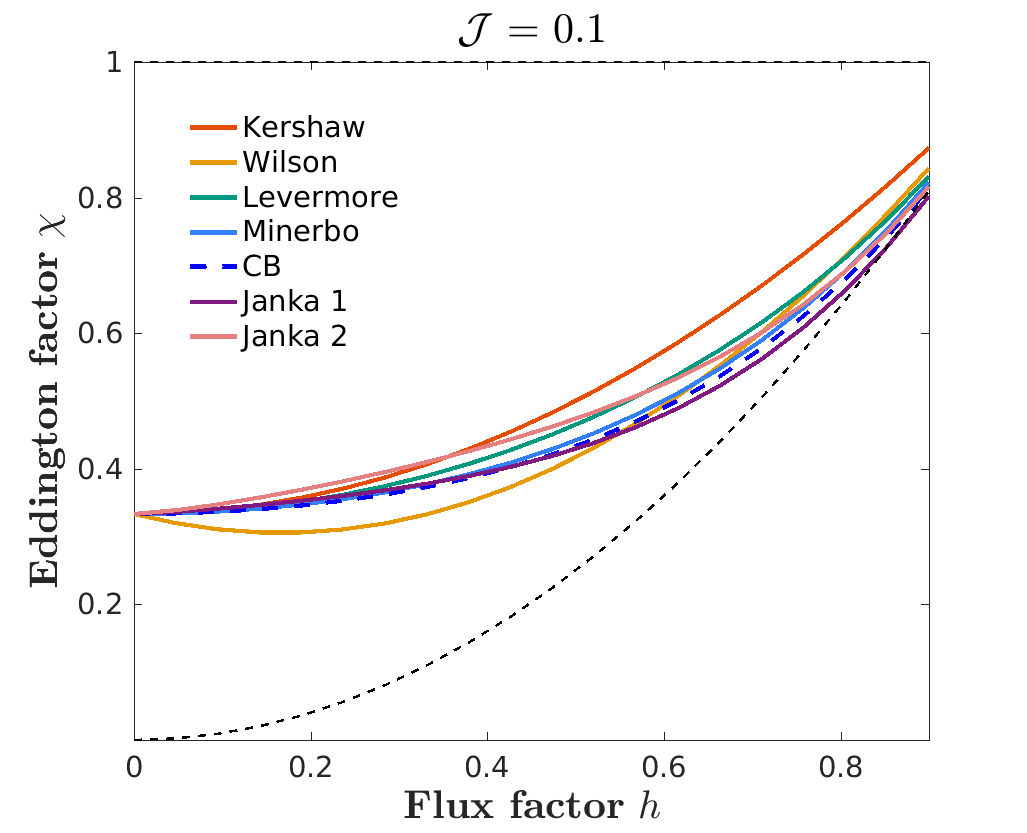
\includegraphics[width=0.5\textwidth]{figures/Closures0_10}
    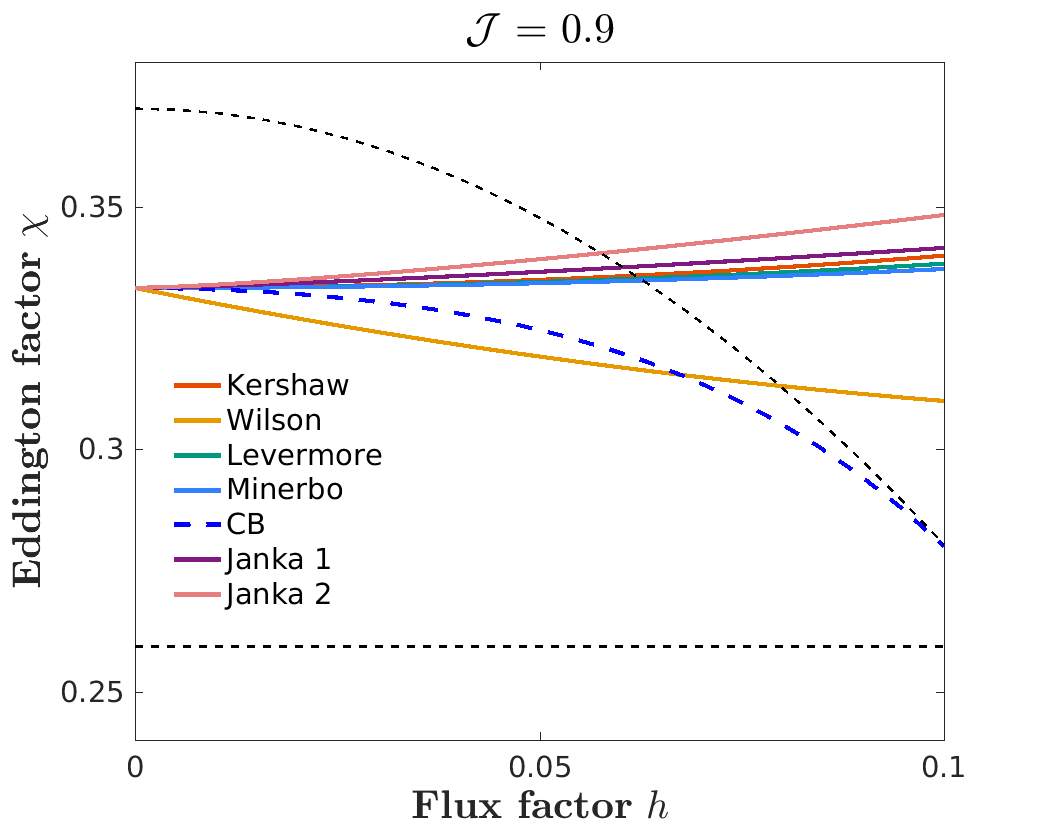
\includegraphics[width=0.5\textwidth]{figures/Closures0_90}
  \end{tabular}
   \caption{Plot of Eddington factors $\chi$ versus flux factor $h$ for different values of $\cJ$ for various algebraic closures: $\cJ=0.1$ (left panel, low occupied) and $\cJ=0.9$ (right panel, high occupied).  In each panel we plot the Eddington factors of Kershaw (red), Wilson (yellow), Levermore (green), Minerbo (light blue), Cernohorsky \& Bludman (blue) and Janka (purple and pink) closures.  We also plot $\chi_{\mbox{\tiny min}}$ and $\chi_{\mbox{\tiny max}}$ defined in Eq.~\eqref{eq:eddingtonFactorBounds} (lower and upper dash black lines, respectively).}
  \label{fig:EddingtonFactorsWithDifferentClosure}
\end{figure}

